%%%%%%%%%%%%%%%%%%%%%%%%%%%%%%%%%%%%%%%%%
% Masters/Doctoral Thesis 
% LaTeX Template
% Version MBE (2022-10-27):
% https://mbe.informatik.uni-siegen.de/
%
% This template was downloaded from:
% http://www.LaTeXTemplates.com
%
% Version 2.x major modifications by:
% Vel (vel@latextemplates.com)
%
% This template is based on a template by:
% Steve Gunn (http://users.ecs.soton.ac.uk/srg/softwaretools/document/templates/)
% Sunil Patel (http://www.sunilpatel.co.uk/thesis-template/)
%
% Template license:
% CC BY-NC-SA 3.0 (http://creativecommons.org/licenses/by-nc-sa/3.0/)
%%%%%%%%%%%%%%%%%%%%%%%%%%%%%%%%%%%%%%%%%

%----------------------------------------------------------------------------------------
%	PACKAGES AND OTHER DOCUMENT CONFIGURATIONS
%----------------------------------------------------------------------------------------

\documentclass[
11pt, % The default document font size, options: 10pt, 11pt, 12pt
%oneside, % Two side (alternating margins) for binding by default, uncomment to switch to one side
singlespacing, % Single line spacing, alternatives: onehalfspacing or doublespacing
%draft, % Uncomment to enable draft mode (no pictures, no links, overfull hboxes indicated)
%nolistspacing, % If the document is onehalfspacing or doublespacing, uncomment this to set spacing in lists to single
liststotoc, % Uncomment to add the list of figures/tables/etc to the table of contents
%toctotoc, % Uncomment to add the main table of contents to the table of contents
%parskip, % Uncomment to add space between paragraphs
%nohyperref, % Uncomment to not load the hyperref package
headsepline, % Uncomment to get a line under the header
%chapterinoneline, % Uncomment to place the chapter title next to the number on one line
%consistentlayout, % Uncomment to change the layout of the declaration, abstract and acknowledgements pages to match the default layout
%anonymous, % MBE: Uncomment to compile a PDF without personal information, so it can be submitted to plagiarism detection tools
]{MastersDoctoralThesis} % The class file specifying the document structure

\usepackage[utf8]{inputenc} % Required for inputting international characters
\usepackage[T1]{fontenc} % Output font encoding for international characters

\usepackage{mathpazo} % Use the Palatino font by default
\usepackage{MnSymbol}


\usepackage[backend=bibtex,style=numeric,natbib=true,maxbibnames=99]{biblatex}

\addbibresource{main.bib} % The filename of the bibliography

\usepackage[autostyle=true]{csquotes} % Required to generate language-dependent quotes in the bibliography



%----------------------------------------------------------------------------------------
%	MARGIN SETTINGS
%----------------------------------------------------------------------------------------

\geometry{
	paper=a4paper, % Change to letterpaper for US letter
	inner=2.5cm, % Inner margin
	outer=3.8cm, % Outer margin
	bindingoffset=.5cm, % Binding offset
	top=1.5cm, % Top margin
	bottom=1.5cm, % Bottom margin
	%showframe, % Uncomment to show how the type block is set on the page
}

%----------------------------------------------------------------------------------------
%	THESIS INFORMATION
%----------------------------------------------------------------------------------------

\thesistitle{Transformation und Analyse von parallelen Datenbankprozessen}{Tranformation and Analysis of Parallel Database Processes } % Your thesis title in german and english, this is used in the title and abstract, print it elsewhere with \detitle and \entitle or \ttitle
\author{Marin \textsc{Bressel}} % Your name, this is used in the title page and abstract, print it elsewhere with \authorname
\keywords{} % Keywords for your thesis, this is not currently used anywhere in the template, print it elsewhere with \keywordnames
\university{Universität Siegen}{University of Siegen} % Your university's name, this is used in the title page and abstract, print it elsewhere with \deunivname and \enunivname or \univname
\chair{Professur für Modellbasierte Entwicklung}{Chair of Model-based Engineering}
\AtBeginDocument{
\hypersetup{pdftitle=\ttitle} % Set the PDF's title to your title
\hypersetup{pdfauthor=\authorname} % Set the PDF's author to your name
\hypersetup{pdfkeywords=\keywordnames} % Set the PDF's keywords to your keywords
}

\begin{document}

%----------------------------------------------------------------------------------------
%	SELECT LANGUAGE
%----------------------------------------------------------------------------------------

\selectlanguage{ngerman} % english for English

\frontmatter % Use roman page numbering style (i, ii, iii, iv...) for the pre-content pages

\pagestyle{plain} % Default to the plain heading style until the thesis style is called for the body content

%----------------------------------------------------------------------------------------
%	TITEL SEITE
%----------------------------------------------------------------------------------------

\begin{titlepage}
\begin{center}

{\scshape\LARGE \univname\par}\vspace{1.5cm}

\vspace*{.03\textheight}

\IfLanguageName{ngerman}{\textsc{\Large Bachelorarbeit \\ im Fach Informatik}}{\textsc{\Large Master/Bachelor thesis \\ in the subject of computer science}}\\[0.4cm] % Thesis type



\vspace*{.03\textheight}

\HRule \\[0.4cm]
{\huge \bfseries \ttitle\par}\vspace{0.5cm}
\HRule \\[1.5cm]
 

\IfLanguageName{ngerman}{vorgelegt von}{submitted by}

\vspace*{.03\textheight}

\textbf{\authorname}
\end{center}

\vspace*{.20\textheight}

\IfLanguageName{ngerman}{\emph{Betreuer:}}{\emph{Supervisors:}}
\vspace{0.5em}

\ifbool{anonymous}{
	\hspace{1em} Anonymous
}{
	% Erstbetreuer
	\hspace{1em} Prof. Dr. M. \textsc{Lochau},\vskip0em
	\hspace{2em}\chairname,\vskip0em
	\hspace{2em}\univname

	% Zweitbetreuer
	\vspace{0.5em}
	\hspace{1em} M. Sc. \textsc{Schüler},\vskip0em
	\hspace{2em}\chairname,\vskip0em
	\hspace{2em}\univname

	\vfill

	% Date

}

\end{titlepage}

%----------------------------------------------------------------------------------------
%	EIDESSTATTLICHE ERKLÄRUNG
%----------------------------------------------------------------------------------------

\begin{declaration}
\IfLanguageName{ngerman}{

%German declaration

\noindent Ich versichere nach § 39 (1) der Einheitlichen Regelungen, meine Arbeit (bei einer
Gruppenarbeit meinen entsprechend gekennzeichneten Anteil der Arbeit) selbständig
verfasst und keine anderen als die angegebenen Quellen und Hilfsmittel benutzt
sowie Zitate kenntlich gemacht zu haben. \\

\vspace{1cm}
\noindent \rule[1em]{15em}{0.5pt} \hfill \rule[1em]{20em}{0.5pt} \\
Ort, Datum \hfill Unterschrift\\}{

%English declaration

\noindent Ich versichere nach § 39 (1) der Einheitlichen Regelungen, meine Arbeit (bei einer
Gruppenarbeit meinen entsprechend gekennzeichneten Anteil der Arbeit) selbständig
verfasst und keine anderen als die angegebenen Quellen und Hilfsmittel benutzt
sowie Zitate kenntlich gemacht zu haben. \\

\vspace{1cm}
\noindent \rule[1em]{15em}{0.5pt} \hfill \rule[1em]{20em}{0.5pt} \\
Ort, Datum \hfill Unterschrift\\}
\end{declaration}

\cleardoublepage


%----------------------------------------------------------------------------------------
%	ABSTRACT / ZUSAMMENFASSUNG: see Abstracts folder
%----------------------------------------------------------------------------------------

\begin{otherlanguage}{ngerman}
\begin{abstract}
% German abstract / Deutsche Zusammenfassung

\todo{Deutsche Zusammenfassung}
\end{abstract}
\end{otherlanguage}
\begin{otherlanguage}{english}
\begin{abstract}
% English abstract / Englische Zusammenfassung

\todo{English abstract}

\end{abstract}
\end{otherlanguage}

%----------------------------------------------------------------------------------------
%	DANKSAGUNG
%----------------------------------------------------------------------------------------

%\begin{acknowledgements}
%Text\ldots
%\end{acknowledgements}

%----------------------------------------------------------------------------------------
%	INHALTSVERZEICHNIS/ABBILDUNGSVERZEICHNIS/TABELLENVERZEICHNIS
%----------------------------------------------------------------------------------------

\tableofcontents % Prints the main table of contents

\listoffigures % Prints the list of figures

\listoftables % Prints the list of tables

\lstlistoflistings % Prints the list of listings

%----------------------------------------------------------------------------------------
%	ABKÜRZUNGSVERZEICHNIS
%----------------------------------------------------------------------------------------

\begin{abbreviations}{ll} % Include a list of abbreviations (a table of two columns)
\textbf{LAH} & \textbf{L}ist \textbf{A}bbreviations \textbf{H}ere\\
\textbf{WSF} & \textbf{W}hat (it) \textbf{S}tands \textbf{F}or\\

\end{abbreviations}

%----------------------------------------------------------------------------------------
%	PHYSKALISCHE KONSTANTEN
%----------------------------------------------------------------------------------------

%\begin{constants}{lr@{${}={}$}l} % The list of physical constants is a three column table
% The \SI{}{} command is provided by the siunitx package, see its documentation for instructions on how to use it
%Speed of Light & $c_{0}$ & \SI{2.99792458e8}{\meter\per\second} (exact)\\
%Constant Name & $Symbol$ & $Constant Value$ with units\\
%\end{constants}

%----------------------------------------------------------------------------------------
%	SYMBOLE
%----------------------------------------------------------------------------------------

%\begin{symbols}{lll} % Include a list of Symbols (a three column table)
%$a$ & distance & \si{\meter} \\
%$P$ & power & \si{\watt} (\si{\joule\per\second}) \\
%Symbol & Name & Unit \\
%\addlinespace % Gap to separate the Roman symbols from the Greek
%$\omega$ & angular frequency & \si{\radian} \\
%\end{symbols}


%----------------------------------------------------------------------------------------
%	THESIS CONTENT - CHAPTERS
%----------------------------------------------------------------------------------------

\mainmatter % Begin numeric (1,2,3...) page numbering

\pagestyle{thesis} % Return the page headers back to the "thesis" style

% Include the chapters of the thesis as separate files from the Chapters folder
% Uncomment the lines as you write the chapters

% Chapter 1


\chapter{Einleitung} % Main chapter title

\label{Chapter1} % For referencing the chapter elsewhere, use \ref{Chapter1} 

%----------------------------------------------------------------------------------------

% Define some commands to keep the formatting separated from the content 
\newcommand{\keyword}[1]{\textbf{#1}}
\newcommand{\tabhead}[1]{\textbf{#1}}
\newcommand{\code}[1]{\texttt{#1}}
\newcommand{\file}[1]{\texttt{\bfseries#1}}
\newcommand{\option}[1]{\texttt{\itshape#1}}

%----------------------------------------------------------------------------------------

\section{Aufbau der Arbeit}
Im Rahmen dieser Arbeit wollen wir ermöglichen parallele Datenbankprozesse sowohl zu analysieren als auch zu Transformieren. Um zu verstehen was genau hier passieren soll und wie eine Mögliche Umsetzung aussehen könnte, müssen wir zunächst einige Begriffe definieren und deren Bedeutung verstehen. Da wir uns im generellen Bereich von Prozessen befinden, muss zunächst erläutert werden was unter einem Prozess zu verstehen ist und auf welche Art von Prozessen wir uns beschränken wollen.
Bei Prozessen handelt es sich um sogenannte reaktive Systeme. Es sind also Systeme, welche auf eine Eingabe warten und je nach Zustand entsprechend reagieren. Hierfür sind in jedem erdenklichen Teil des Alltags Beispiele zu finden. Es kann sich um Komplexe Prozesse in Computerspielen oder Betriebssystemen handeln, oder auch um ganz einfache Abläufe im Alltag. Ein einfaches Beispiel ist in Abbildung 1.1 dargestellt. Hier ist der Tagesablauf eines gewöhnlichen Angestellten einer beliebigen Firma zu sehen.\\
Wir wollen uns in dieser Arbeit zum größten Teil mit Abläufen von Geschäftsprozessen auseinandersetzen. Damit sind unter anderem jene Abläufe gemeint, die innerhalb von beispielsweise Firmen passieren. Es kann sich hier um viele Verschiedene Abläufe handeln.\\
\begin{figure}
\centering
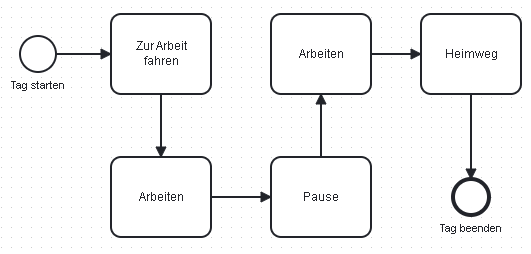
\includegraphics[scale=0.7]{Figures/Einleitungbsp1}
\decoRule
\caption[Alltag eines Mitarbeiters]{Alltag eines Mitarbeiters}
\label{fig:Task}
\end{figure}
Ein passendes Beispiel ist in Abbildung 1.2 zu sehen. Es handelt sich hier um einen Prozess, welcher auf einer beliebigen Internetseite abläuft. Wir beschränken uns hier der Einfachheit halber auf den Prozess des Erstellens eines Accounts. Also auf den Registrierungsprozess. In unserem Beispiel muss der Nutzer auf der Homepage zunächst den Button „Registrieren“ drücken. Er wird im Anschluss auf die korrekte Internetseite weitergeleitet und hat da die Möglichkeit seine Anmeldedaten anzugeben. Nun muss die Korrektheit der Daten geprüft werden. Im Anschluss wird der Nutzer erstellt und wieder auf die Homepage zurück geleitet.\\
\begin{figure}
\centering
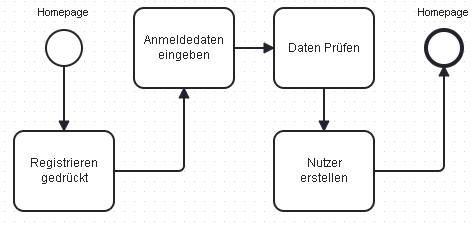
\includegraphics[scale=0.7]{Figures/Einleitungbsp2}
\decoRule
\caption[Einfacher Registrierungsprozess]{Einfacher Registrierungsprozess}
\label{fig:Task}
\end{figure}
Solche und ähnliche Prozesse laufen in jeder erdenklichen Firma ab und unterscheiden sich sehr stark voneinander in Komplexität und Inhalt.\\
Bei dem zweiten Begriff, der verstanden werden muss handelt es sich um BPMN (Business Proccess Moddeling Notation). Hierbei handelt es sich um eine Standardisierte Modellierungssprache. Die in den Abbildungen 1.1 und 1.2 dargestellten Beispiele wurden bereits in BPMN dargestellt. Eine Detailliertere Beschreibung erfolgt im Abschnitt 2.1 doch die wichtigsten Features sollen hier schon einmal erwähnt werden. Sie sind, neben den Aktivitäten welche durch abgerundete Rechtecke dargestellt werden und der Konkatenation dieser Aktivitäten durch die Pfeile, die sogenannten Gateways, welche durch Rauten mit einem Entsprechenden Symbol dargestellt werden. Ist ein „X“ in die Raute geschrieben so handelt es sich um ein Exklusives OR-Gateway. Hier kann exakt eine der folgenden Pfade ausgeführt werden. Findet man ein „+“ vor, so liegt ein paralleles Gateway vor. Hier werden alle Pfade gleichzeitig ausgeführt. Ein weites paralleles Gateway vereinigt die Pfade dann wieder. An dieser Stelle wird also gewartet, bis alle parallelen Aktivitäten durchgeführt worden sind. Diese Arbeit beschäftigt sich ausschließlich mit Prozessen in BPM.Es wird allerdings nur eine Teilmenge benutzt.

Zuletzt muss nun noch erläutert werden zu was diese Prozesse transformiert werden sollen. Hierzu müssen wir den Begriff einer Prozessalgebra genauer erläutern. Bei einer Prozessalgebra handelt es sich nun um einen mathematischen Kernkalkül zur Darstellung von Prozessen. Es bietet also eine Möglichkeit die selben Prozesse durch eine Art Formeln darzustellen. Wir wollen in dieser Arbeit eine Prozessalgebra verwenden, welche auf ACP basiert.  Zum besseren Verständnis möchte ich auch hier die wichtigsten Features von ACP erläutern. Ähnlich zu BPMN gibt es Möglichkeiten zur Darstellung von Konkatenation, oder-Zweigen und auch Parallelen Zweigen. Eine Aktivität wird durch einfach als Variable dargestellt. Wie diese genannt wird, ist zunächst irrelevant. Eine Konkatenation wird durch ein \textit{*} dargestellt. Ein Exklusiver oder-Zweig wird durch ein \textit{+} und ein paralleler Zweig durch \textit{||} dargestellt. Würde man das Beispiel in Abbildung 1.2 also nun nach ACP überführen, so würde ein Mögliches Ergebnis wie folgt aussehen: 

$P:=Start*RegestrierenGedrückt*AnmeldeDatenEingeben*DatenPrüfen*NutzerErstellen'Homepage $


\section {Ziel der Arbeit}

Das Ziel dieser Arbeit ist es nun Programm zu entwickeln, welches ein BPMN Diagramm einlesen und dieses zu einer Formel in der Prozessalgebra überführen kann. Es soll also ein Mapping von BPMN nach ACP erfolgen. 

Der Zweck dieser Arbeit wird erkennbar, sobald Daten in form einer relationalen Datenbank für den Prozess relevant werden. BPMN bietet hier nur schwammige und unübersichtliche Methoden die Daten darzustellen. Es erweist sich also als schwierig zu Analysieren und zu verifizieren, was genau mit den Daten passiert. Zudem lässt BPMN zu viel Raum für Interpretation. Es wird viel mit Kommentaren gearbeitet und was genau in einem bestimmten Abschnitt des Prozesses passiert ist in vielerlei Hinsicht offen zur Interpretation. ACP ist etwas Strukturierter. Zudem bietet die Variante die von uns genutzt wird die Möglichkeit mit einer konkreten Datenbank zu kommunizieren und Anweisungen auf dieser auszuführen. Aus diesem Grund ist ein weiteres Ziel dieser Arbeit, die passenden Datenbankanweisungen zu dem jeweiligen Prozess auf einer relationalen Datenbank auszuführen.





% Chapter 1

\chapter{Grundlagen} % Main chapter title

\label{Chapter2} % For referencing the chapter elsewhere, use \ref{Chapter1} 

%----------------------------------------------------------------------------------------

% Define some commands to keep the formatting separated from the content 


%----------------------------------------------------------------------------------------



Das folgende Kapitel dient dazu die in der Einleitung genannten Begriffe und Prinzipien genauer zu erläutern. Wir wollen also zunächst BPMN und die Bestandteile der Modellierungssprache genauer betrachten. Hierzu werden wir jedes Element einzeln betrachten und dadurch stück für Stück ein passendes Beispiel erstellen. Dieses Beispiel wird auch im Rest der Arbeit Relevanz finden. 
Im Anschluss wird dann die verwendete Prozessalgebra genauer betrachtet. Auch hier wollen wir jeden Bestandteil des Modells im Detail erläutern.
\section{BPMN}
Wie in der Einleitung bereits erwähnt, dient BPMN der graphischen Darstellung von Business Prozessen. In BPMN werden diese Prozesse in einzelne Aktivitäten oder Aufgaben unterteilt und dann in der richtigen Reihenfolge aufgezeichnet. Es gibt unterschiedliche Möglichkeiten Verzweigungen, Abhängigkeiten und Ähnliches zu Modellieren doch zum größten Teil basiert alles auf der korrekten Aneinanderreihung dieser Aktivitäten.
\subsection{Erste Schritte - Events und Aktivitäten}
Im folgenden Abschnitt schauen wir uns also die von uns verwendete Teilmenge der Modellierungssprache BPMN an. Hierzu möchten wir zunächst einen einführenden Prozess als Beispiel betrachten. Für alle möglichen Homepages und Websites von unterschiedlichen Firmen und Anbietern können Konten erstellt werden. Diese dienen zur Wiedererkennung eines Kunden oder Mitarbeiters. In diesem Abschnitt wollen wir ein BPMN-Diagramm erstellen, welches den Registrierungsprozess auf einer solchen Website darstellen könnte. Wir werden die Modellierungssprache hierzu aufteilen und jeden Bestandteil der Sprache anhand des Beispiels einzeln erläutern, sodass wir am ende dieses Abschnittes ein erstes, vollständiges Diagramm vorfinden.\\
Die von uns genutzte Teilmenge kann in einzelne Blöcke eingeteilt werden. Diese können in zwei Gruppen unterteilt werden. Die Basic Blocks und die Flow Blocks. Des Weiteren kann unterschieden werden zwischen \textit{Leaf Blocks} und \textit{Nonleaf Blocks}. Alle Nonleaf Blocks bestehen aus beliebig vielen Leaf Blocks. Es existieren genau zwei für uns relevante Leaf Blocks, welche wir hier zunächst erwähnen möchten, um deren Funktion genauer zu erläutern. Die unterschiedlichen Blöcke sind jeweils durch sogenannte \textit{sequnce flows} verbunden. Diese werden dargestellt durch eine durchgezogene Linie mit einem ausgefüllten Pfeil am Ende. Sie verdeutlichen den Fluss des Diagrammes. Jeder Block hat einen eingehenden und einen ausgehenden Flow. Um zu verdeutlichen in welchem Zustand der Prozess sich zu einem bestimmten Zeitpunkt befindet, verwenden wir sogenannte Token. Diese beinhalten keine Daten, sondern stellen nur dar, welcher Teil des Prozesses gerade aufgeführt wird. Beim Ausführen des Prozesses wird ein Token immer in Richtung der Sequence Flows weitergegeben.\\
Bei dem \textit{Task Block} und dem \textit{Event Block} handelt es sich um die beiden relevanten leaf-Blocks. Beide Blöcke werden durch den Namen bereits gut erklärt. Der Task Block, welcher durch ein abgerundetes Rechteckt dargestellt wird, ist repräsentativ für eine beliebige Aufgabe. Diese Aufgaben benötigen in jedem Fall Zeit, um ausgeführt zu werden. Er kann durch einen Text in der Mitte des Rechtecks beliebig benannt werden. Diese Aufgaben können jede erdenkliche Form annehmen. Eine Mögliche Aufgabe ist in Abbildung 2.1 dargestellt. Es handelt sich um das Eingeben der Anmeldedaten.Hierbei handelt es sich um eine Aufgabe die Zeit beansprucht und vom Nutzer ausgeführt wird. Sie ist offensichtlich relevant für unser Beispiel.\\
\begin{figure}
\centering
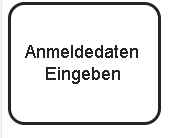
\includegraphics[scale=1.0]{Figures/Beispiel1}
\decoRule
\caption[Einfache Task]{Einfache Task - Anmeldedaten eingeben}
\label{fig:Task}
\end{figure}Bei dem zweiten Leaf Block handelt es sich nun um sogenannte Events. Events werden durch einen Kreis dargestellt. Anders als die Aufgaben passieren Events sofort. Es gibt unterschiedliche Typen, welche durch unterschiedliche Variationen eines Kreises dargestellt werden. Für uns relevant sind allerdings nur sogenannte \textit{catching Events}.  Erreicht der Token ein solches Event, wird gewartet bis das erwartete Event auftritt und erst dann wird der Token weitergeschickt. Auch unter den catching Events gibt es drei grundsätzliche Unterscheidungen. Die einfachsten Variationen sind sogenannte Startevents, welche einen Prozess Starten und durch einen einfachen dünn gezeichneten Kreis dargestellt werden und die Endevents, welche den Prozess terminieren und durch einen einfachen dick gezeichneten Kreis dargestellt werden.\\
Durch die uns nun bekannten Bausteine, ist es uns möglich einen ersten Prozess aufzubauen und in BPMN zu Modellieren. In Abbildung 2.2 sehen wir ein Beispiel für den ersten und einfachsten nonleaf-Block. Den \textit{Prozess-Block}. Dieser besteht aus einem Start- und einem Endevent. Zwischen den beiden Events liegt mindestens ein Task-Block und beliebig viele Event Blocks. Der Prozess in unserem Beispiel startet, indem ein Nutzer die Seite besucht und einen neuen Account anlegen möchte. Dieser wird zunächst auf eine Seite weitergeleitet, welche seine Anmeldedaten abfragt. Diese muss er dann in der ersten Aufgabe eingeben. Die zweite Aufgabe besteht nun darin den neuen Nutzer mit seinen eben angegebenen Daten in die vorhandene Datenbank einzutragen. Sobald diese Aufgabe erledigt ist, endet der Prozess und ein neuer Nutzer wurde erfolgreich angelegt.\\
\begin{figure}
\centering
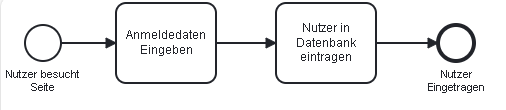
\includegraphics[scale=1.0]{Figures/Beispiel2}
\decoRule
\caption[Prozess Block]{Erster Vollständiger Prozessblock}
\label{fig:Task}
\end{figure}Events können allerdings auch während eines Prozesses auftreten. Wollen wir in unserem Beispiel einführen, dass die Startseite besucht werden kann, ohne, dass direkt auf die Nutzer anlegen Seite weitergeleitet wird, so können wir eine neue Aufgabe und ein fangendes Event einführen. Abbildung 2.3 zeigt diesen Prozess. Er startet, indem ein Nutzer die von uns erstellte Website besucht. Im nächsten Schritt wartet das catching Event, bis der Nutzer sich dazu entscheidet einen neuen Account anzulegen. In Folge dessen verhält sich der Prozess so, wie im Beispiel aus Abbildung 2.2. Events welche während dem Prozess auftreten werden \textit{Intermediate Events} genannt.
\begin{figure}
\centering
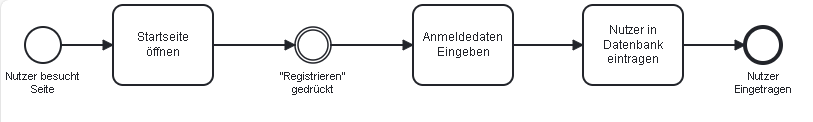
\includegraphics[scale=0.6]{Figures/Beispiel3}
\decoRule
\caption[Intermediate Events]{Beispiel für ein intermediate Event}
\label{fig:Task}
\end{figure}
\subsection{Mögliche Verzweigungen}
In nun folgenden Abschnitt wollen wir uns mit Möglichkeiten beschäftigen den Sequenzfluss zu verzweigen. Hierzu bietet BPMN einige sogenannte \textit{Gateways}. Um Gateways darzustellen, werden Rauten verwendet. Unterschiedliche Gateways haben unterschiedliche Symbole in den Rauten eingezeichnet. Sie sind dafür da, den Verlauf des Prozesses aufzuteilen und wieder korrekt zusammenzufügen. Wenn ein Gateway den Verlauf des Prozesses aufspaltet, so muss immer ein zweites Gateway den Verlauf wieder zusammenfügen. Eine Ausnahme hierfür wäre, wenn der Prozess in einer Verzweigung durch ein Endevent terminiert.\\
Um unser bislang erarbeitetes Beispiel etwas realitätsnaher zu gestalten, wollen wir eine neue Funktion einführen. Offensichtlich soll unsere Seite mehr Funktionen anbieten als neue Nutzer anzulegen. Die nächste logische Erweiterung ist eine Möglichkeit für bereits bestehende Kunden sich mit ihren vorhandenen Anmeldedaten einzuloggen. Hier spielt die erste Verzweigungsmöglichkeit eine Rolle. Da ein Nutzer immer entweder ein bestehendes Konto besitzt oder ein neues erstellen möchte, wird in jedem Durchlauf des Prozesses nur eine dieser Aktionen durchgeführt. Hier kann ein XOR-Gateway genutzt werden. Es ist zu erkennen durch ein \textit{X} in der Raute. Es bietet die Möglichkeit zwischen unterschiedlichen Pfaden zu wählen. Im Beispiel aus Abbildung 2.4 sehen wir eine mögliche Verwendung für dieses Gateway. Nachdem der Nutzer auf der Startseite den entsprechenden Button betätigt, wird er entweder zur Anmeldung oder zur Registrierung weitergeleitet. In beiden Fällen muss er seine Daten angeben. Je nachdem in welchem Teil wir uns befinden muss der Nutzer in der Datenbank eingetragen werden oder die Anmeldedaten müssen geprüft werden. Im Anschluss werden die zwei Äste wieder zusammengeführt und der Nutzer wird mit seinem zugehörigen Account auf der Seite angemeldet. Beim Zusammenführen der Äste, wartet das Gateway auf genau einen Token und gibt diesen dann weiter an das nächste Objekt. In diesem Beispiel ist der erste Flow-Block zu erkennen. Wird der Verlauf des Prozess durch ein XOR-Gateway aufgespalten und wieder zusammengeführt, so bilden alle Elemente innerhalb dieser Verzweigung im sogenannen \textit{Exclisive-choice-Block}. Abbildung 2.4 zeigt außerdem eine Mögliche Variante des XOR-Gateways. Wenn der Nutzer einen vorhandenen Account anmelden möchte, aber inkorrekte Anmeldedaten eingibt, so wird er auf die Startseite zurückgeleitet. Das XOR-Gateway kann also auch für Loops verwendet werden. Hier ist zu erkennen, dass das zusammenführende Gateway durchaus auch vor dem aufspaltenden Gateway liegen kann. Es ist zusätzlich möglich auch mehr als zwei Ausgänge an das Gateway anzubinden.\\
\begin{figure}
\centering
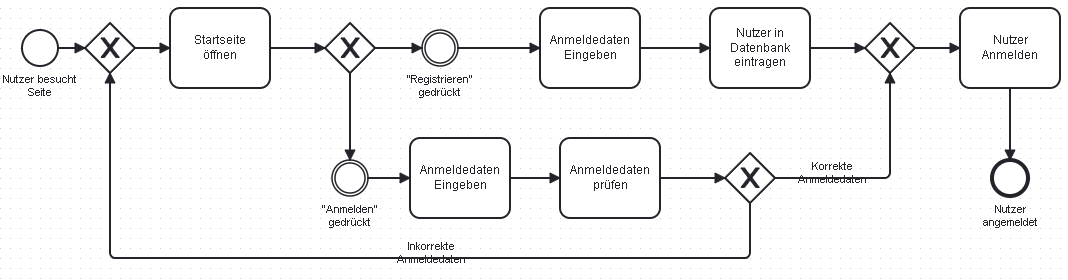
\includegraphics[scale=0.5]{Figures/Beispiel5}
\decoRule
\caption[XOR-Gateway]{Exclusive Entscheidung - Das XOR-Gateway}
\label{fig:Task}
\end{figure}Wir wollen nun ein weiteres Feature in unser Diagramm einfügen. Nachdem ein neuer Account erstellt wurde, soll dieser Nutzer nach wie vor angemeldet und auf die Homepage weitergeleitet werden. Zusätzlich soll er gleichzeitig auch für den Newsletter der Website eingetragen werden. Hierzu können wir ein weiteres Gateway nutzen. Das parallele Gateway wird in Abbildung 2.5 das erste Mal gezeigt. Es wird ebenfalls durch eine Raute dargestellt. Diese enthält allerdings ein + in ihrem Inneren. An diesem Gateway wird der Verlauf des Prozesses wieder aufgespalten. Anstelle von nur einem Strang werden hier aber alle Gelichzeitig ausgeführt. Das zusammenführende Gateway muss desshalb nicht blind den ersten Token weiterschicken, den es erhält, sondern wartet bis an allen Eingängen ein Token vorliegt, fügt diese wieder zusammen und gibt dann den Token weiter an das nächste Objekt. Hier können Schwierigkeiten auftreten, falls ein paralleler Zweig in einem Endevent endet. Bei der Modellierung eines Diagrammes muss dies also verhindert werden. Insgesamt spricht man hier von einem \textit{Parallel Block}\\
\begin{figure}
\centering
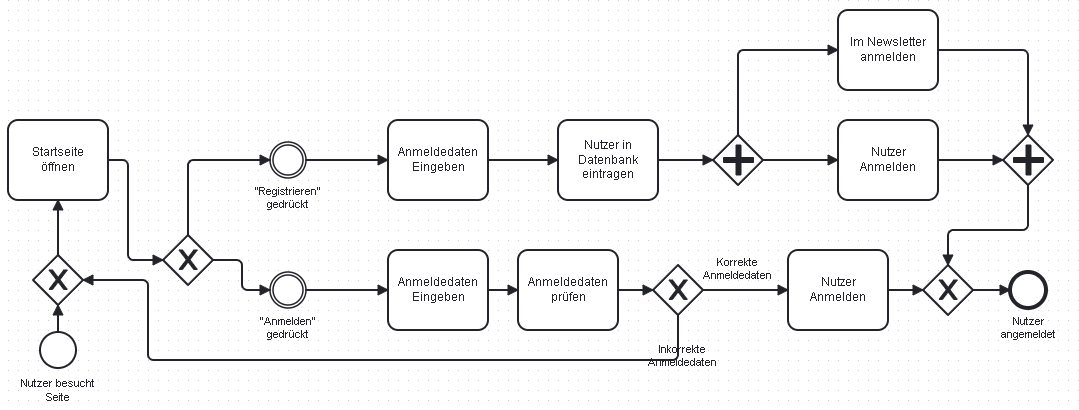
\includegraphics[scale=0.5]{Figures/Beispiel6}
\decoRule
\caption[Paralell-Gateway]{Parallele Ausführung - Das Paralell-Gateway}
\label{fig:Task}
\end{figure}
\subsection{Subprozesse und weitere Elemente}
Der letzte Block, welcher von uns genauer betrachtet wird ist der \textit{subprocess-Block}. Auch dieser wird bereits durch den Namen gut beschrieben. Zur vereinfachten Darstellung, kann ein Teil von einem Prozess als ein unterprozess zusammengefasst werden. In Abbildung 2.6 ist also der selbe Prozess dargestellt wie der in Abbildung 2.5. Hier wurde der Teil des Prozesses, in dem ein Nutzer registriert wird zu einem Subprocess zusammengefasst. In Abbildung 2.7 findet sich zudem eine Alternative Darstellung dieses Blockes. Hier ist zu sehen, dass der Subprozess auch als einzelnes Elemt auftauchen kann. An der Stelle wird dann eine referenz zu einem Prozess gemacht. Dieser enthält die Elemente die von dem Subprocess ausgeführt werden. In dieser Abbildung ist zustätzlich noch eine Übersicht über alle für uns relevante Elemente zu finden.\\
\begin{figure}
\centering
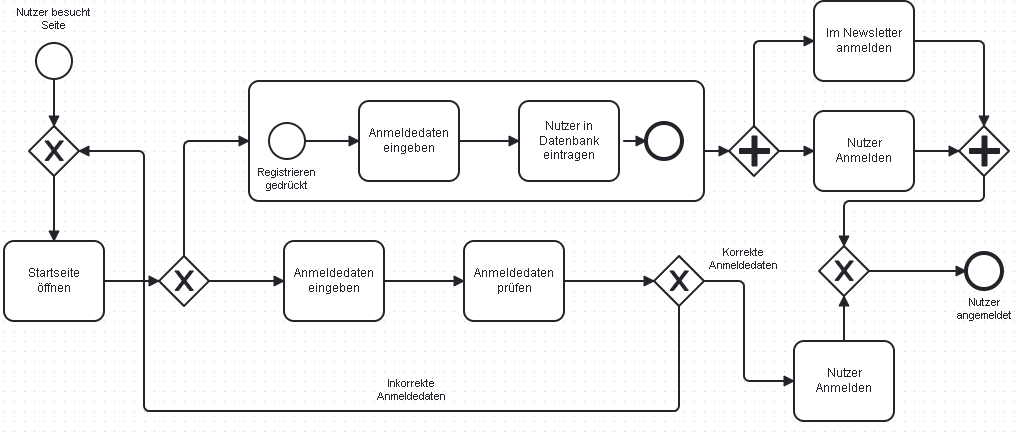
\includegraphics[scale=0.5]{Figures/Beispiel7}
\decoRule
\caption[Subprocess Block]{Subprocess Block - Prozesse innerhalb von Prozessen}
\label{fig:Task}
\end{figure}Zuletzt möchten wir nun jene Elemente beschreieben, die für unsere Arbeit nicht wichtig werden. Hierbei handelt es sich zum großteil um Varianten der uns bekannten Bausteine. Neben den Exclusive und Parallel Gateways existieren noch so genannte Event-based Gateways. Diese entscheiden anhand eines eintreffenden Events, wleche Aktion ausgefürt wird. 
Die Task blocks lassen sich durch Symbole in der oberen linken Ecke genauer spezifizieren. Hier wird unterschieden zwischen User task, Service task, Business rule task und Script task. Auch unter den Events kann genauer spezifiziert werden. Für alle catching events sind throwing events vorhanden und auch unter diesen gibt es unterschieldiche Typen wie Message Evens oder timer Events. Zudem gibt es eine Möglichkeit Datenflüsse darzustellen durch eine sogenannte \textit{Date object reference} oder eine \textit{Data store reference}. Zuletzt bietet BPMN eine möglichkeit verschiedene Teilnehmer einer Prozesses darzustellen. Sogenannte \textit{pools} und \textit{lanes} können genutzt werden um Gruppen und auch einzenle Teilnehmer innerhalb dieser Gruppen darzustellen.\\
\begin{figure}
\centering
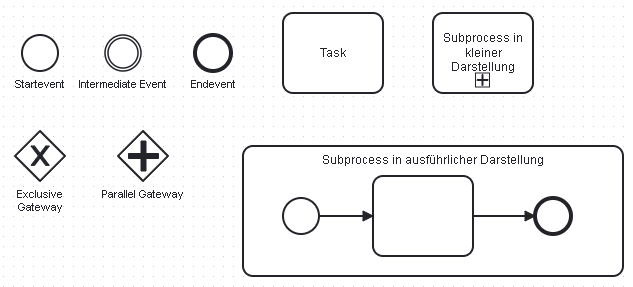
\includegraphics[scale=0.5]{Figures/Alleblocke}
\decoRule
\caption[Alle Elemente]{Alle von uns genutzten Elemente}
\label{fig:Task}
\end{figure}
\section {Prozessalgebra - ACP}
Nachdem wir die wichtigsten Bestandteile der Modellierungssprache BPMN eingeführt haben, wollen wir uns nun mit der Prozessalgebra ACP beschäftigen und diese mit ihren einzelnen Bestandteilen genauer erläutern.\\
Parallel zu den Tasks in BPMN sprechen wir hier von sogenannten Aktionen. Diese werden klein geschrieben und können ansonsten beliebig benannt werden. Auch Prozesse und Sub-prozesse werden hier angewendet. Die Syntax für einen Prozess welcher eine beliebige Aktion ausführt ist durch P::=v gegeben. Ein mögliches Beispiel ist auch hier wieder das Registrieren eines neuen Nutzers. P::=nutzerRegistrieren beschreibt also den Prozess P welcher die Aktion nutzerRegistrieren ausführt. Analog dazu können auch Subprozesse dargestellt werden. P::=K beschreibt den Prozess P welcher daraus besteht die Prozess K auszuführen. Dies kann zur vereinfachten Darstellung von ausführlicheren Prozessen oder zur Darstellung von Rekursion genutzt werden.\\
Ähnlich wie bei BPMN können Prozesse und Aktionen in ACP konkateniert werden. Hierzu wird der *-Operator verwendet. Der Prozess, welcher in Beispiel 2.2 als BPMN Diagramm dargestellt ist, kann also durch P::=anmeldedatenEingeben*nutzerInDbEintragen in ACP dargestellt werden. Hier fällt auf, dass sowohl das Startevent als auch das Endevent nicht in der Formel enthalten sind. In ACP gibt es generell kein Äquivalent zu den Events.\\
Anders als bei den Events, gibt es für die Gateways welche in Abschnitt 2.1 erläutert wurden auch in ACP Darstellungsmöglichkeiten. Zunächst wollen wir die XOR-verknüpfung erklären. Diese wird durch den +-Operator dargestellt. Auch hier kann ein zuvor durch BPMN modelliertes Beispiel verwendet werden. Wir können hierzu das in Beispiel 2.4 gezeigt Diagramm in eine Formel in ACP umwandeln. P::=sO*((aE*nE)+(aE*aP))*nA\\
Die Klammern können so interpretiert werden, dass die umschlossenen Terme zusammenhängen. Es wird in dem Beispiel also entweder (aE*nE) oder (aE*aP) ausgeführt.\\
Außerdem wurden folgende Abkürzungen genutzt.\\
sO -> Startseite Öffnen\\
aE ->Anmeldedaten Eingeben\\
nE ->Nutzer Eintragen (In DB)\\
aP ->Anmeldedaten Prüfen\\
nA ->Nutzer Anmelden\\
Als nächstes wollen wir nun veranschaulichen wie das Parallel-Gateway aus BPMN in APC umgesetzt wird. Hierzu gibt es drei unterschiedliche sogenannte Merge-Operatoren. Diese sollen hier nun einzeln erklären.
Zunächst betrachten wir den regulären Merge-Operator. Dieser wird durch ein || dargestellt und beschreibt das parallele Ausführen zweier Prozesse. Sollte der Prozess P also durch P::=Q||R beschrieben werden, so ist egal welcher der beiden Subprozesse Q oder R zuerst eine Aktion ausführt.\\
Als nächstes beschreiben wir nun den Left-Merge-Operator. Dieser wird durch ein $\leftMerge$ dargestellt. Auch hier werden beide Subprozesse ausgeführt. Es muss allerding zuerst der Linke der beiden eine Aktion ausführen. Im Anschluss verhält sich der Operator genauso wie der reguläre Merge-Operator. Zuletzt betrachten wir den Communication-Merge-Operator, welcher durch ein | dargestellt wird. Hier werden beide Subprozesse gleichzeitig in einem Schritt ausgeführt.
\section{Datenbanken}
Im folgenden Kapitel werden nun Relationale Datenbanken genauer beschrieben. Wir betrachten zunächst ein Relationsschema  $\mathcal{R} = \{R_1/a_1,…,R_n/a_n\}$. Dies beinhaltet eine Menge an Relationen $R_i$, welche jeweils eine zugehörige Stelligkeit $a_1$ besitzen. Dieses Schema beschreibt unsere Datenbank. Jede Relation $R_i$ aus  $\mathcal{R}$ kann als Tabelle der Datenbank angesehen werden. \\
Auch hier findet das in den Vorherigen Abschnitten verwendete Beispiel Anwendung. Um den Registrierungs- und Anmeldeprozess umsetzen zu können, müssen zumindest die Kontodaten jedes Nutzers gespeichert werden. Diese beinhalten in unserem Beispiel lediglich den Nutzernamen und das Passwort. Unser Beispiel benötigt also nur eine Tabelle. Das bedeutet, dass in unserem Relationsschema nur eine Relation hinterlegt ist. Diese könnte beispielsweise den Namen Nutzer tragen. Da die Tabelle Nutzer aus den zwei Spalten Nutzername und Passwort besteht beträgt die Stelligkeit der Relation zwei. Das Relationsschema aus unserem Beispiel lautet also $\mathcal{R}_1=\{Nutzer/2\}$. \\
Zusätzlich definieren wir den Begriff der Domäne ${\Delta}$ einer Datenbank als jene zählbar unendliche Menge, welche sämtliche Datentypen enthält, die in der jeweiligen Datenbank vorkommen können. Sie beschränkt sich in unserem Beispiel also auf alle Strings. \\
Eine Instanz $\mathcal{I}$ einer Datenbank ist ebenfalls als eine Menge zu betrachten. Diese Menge enthält sämtliche Daten, die zu einem gewissen Zeitpunkt in der Datenbank abgespeichert werden. Diese Daten werden in Form von Tupeln abgespeichert. Ein Tupel enthält jeweils den Namen der jeweiligen Relation, sowie die Daten eines Elements. Auch hier dient das oben bereits verwendete Beispiel gut zu Veranschaulichung. Befindet beispielsweise ein Nutzer mit dem Nutzernamen \textit{Marin} und dem Passwort \textit{Test} in der Datenbank, so ist $\mathcal{I}_1 = \{(Nutzer, Marin, Test)\}$. Wird nun ein weiterer Nutzer mit dem Nutzernamen \textit{Max} und dem Passwort \textit{pw} hinzugefügt, so wird $\mathcal{I}$ um das Tupel (Nutzer, Max, pw) erweitert. Also ist $\mathcal{I}_2 =\{(Nutzer, Marin, Test), (Nutzer, Max, pw)\}$. Eine Alternative Schreibweise ist durch $\mathcal{I}_2 = \{Nutzer(Marin, Test), Nutzer(Max, pw)\}$ gegeben. Der Name der Relation kann also auch außerhalb der Klammern stehen.\\
In Abbildung 2.8 ist zur veranschaulichung eine Tabelle zu sehen, welche die Inhalte von $\mathcal{I}_2$ überscihtlicher darstellen soll.\\
\begin{figure}
\centering
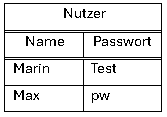
\includegraphics[scale=1]{Figures/Tabelle1}
\decoRule
\caption[Tabelle1]{$\mathcal{I}_2$ graphisch dargestellt}
\label{fig:Task}
\end{figure}Wollen wir die Datenbank nun um eine Weitere Tabelle erweitern, welche beispielsweise zwei Nutzer durch eine Freundschaft verknüpft und zusätzlich speichert seit wie vielen Jahren diese Freundschaft besteht, so wird kann das gegebene Schema $\mathcal{R}_1$ um \textit{Freuzndschaft/3} erweitert werden. Also $\mathcal{R}_2=\{Nutzer/2, Freundschaft/3\}$ dei drei Attribute der Relation Freundschaft sind hierbei Freund\_1, Freund\_2 und Dauer. Das Attribut Dauer beschreibt seit wie vielen Jahren eine Freundschaft besteht und wird als Integer angegeben. Durch diese Änderung wird die Domäne ${\Delta}$ zusätzlich um sämtliche Integer erweitert. 
Fügen wir nun eine Freundschaft zwischen \textit{Max} und \textit{Marin}, welche seit 0 Jahren besteht der Datenbank hinzu, so wird  $\mathcal{I}$ um das Tupel (Freundschaft, Max, Marin, 0) erweitert. Also $\mathcal{I}_3$= \{Nutzer(Marin, Test), Nutzer(Max, pw),Freundschaft(Max, Marin, 0)\}. Abbildung 2.9 zeigt die Instanz in Form von Tabellen.\\
\begin{figure}
\centering
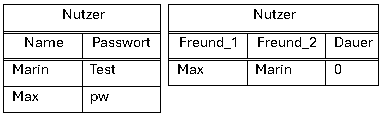
\includegraphics[scale=1]{Figures/Tabelle2}
\decoRule
\caption[Tabelle2]{$\mathcal{I}_3$ graphisch dargestellt}
\label{fig:Task}
\end{figure}Das sogenannte  \textit{Universum} enthält alle möglichen Instanzen in Bezug auf das Schema und der Domäne. $\mathcal{I}_1$, $\mathcal{I}_2$ und $\mathcal{I}_3$ sind also Elemente des Universums.\\
Nun wollen wir betrachten, wie Datenbanken manipuliert werden können.\\
Hierzu müssen wir zunächst betrachten, wie Daten aus der Datenbank ausgelesen werden können.\\
Dazu nutzen wir sogenannte Queries. Diese werden in FOL ausgedrückt. Hierzu definieren wir zunächst eine Menge $VARS = \{u1,…,un\}$. Diese Menge besteht aus Variablen, welche alle Werte aus ${\Delta}$ annehmen können. Zusätzlich bildet eine Substitution ${\sigma}$ alle Variablen auf Vars auf werte in ${\Delta}$ ab. \\
 Eine Query ${\phi}$ ist durch folgende Syntax gegeben: \\
${\phi}$ ::= true | R(u1, . . . , ua) | ${\neg}{\phi}$ | ${\phi}$1 $\wedge$ ${\phi}$2 | $\exists$u.${\phi}$ | u1 = u2 \\
Wir wollen nun die Semantik dahinter erläutern.
\begin{itemize}
\item Für ${\phi}$ ::= true besteht die Query in jedem Fall.
\item Für ${\phi}$ ::= R(u1, . . . , ua) besteht die Query, falls das Tupel R(e1, … ,ea) in I vorliegt. Hierbei ist ei=${\sigma}$(ui) für alle i: 1 </= i </= a.
\item Für ${\phi}$ ::=${\neg}$ Q besteht die Query, falls Q nicht bestehen würde. 
\item Für ${\phi}$ ::= Q1 $\wedge$ Q2 besteht die Query, wenn Q1 und Q2  bestehen würden
\item Für ${\phi}$ ::= u1 = u2  besteht die Query, wenn ${\sigma}$(u1)=${\sigma}$(u2)
\item Für ${\phi}$::= $\exists$u.Q besteht die Query, wenn in der aktuellen Instanz der Datenbank ein Element existiret, welches durch eine Substitution  ${\sigma}$' auf u abgebildet werden kann. 
\end{itemize}
Die Manipulation einer Datenbank besteht aus drei Phasen. Zunächst muss ein eine Query, welche wir als Guard bezeichnen bestehen. Im Anschluss kann die Aktion ausgeführt werden. Die Aktion besteht aus dem löschen eines Elements und dem Hinzufügen eines Elements. Ein Element beschreibt dabei ein Tupel in der Menge $\mathcal{I}$ Hier ist anzumerken, dass es keine Möglichkeit gibt Inhalte der Datenbank zu ändern. Möchte also ein Nutzer sein Passwort ändern, so wird zuerst in einem Schritt der jeweilige Nutzer entfernt und im nächsten Schritt ein neuer Nutzer mit dem veränderten Passwort der Datenbank hinzugefügt.









 
%% Chapter Template

\chapter{Mapping} % Main chapter title

\label{Chapter3} % Change X to a consecutive number; for referencing this chapter elsewhere, use \ref{ChapterX}

%----------------------------------------------------------------------------------------
%	SECTION 1
%----------------------------------------------------------------------------------------
Das folgende Kapitel soll erläutern wie sich beliebige BPMN Diagramme am besten auf ACP Formeln mappen lassen. Es gbt einige unterschiedliche möglichkeiten dieses Mapping durchzuführen. Hier soll erläutert werden wie sich unser Programm verhalten soll und das eine angebrachte lösung darstellt.
\section{Parallelen und Unterschiede}\label{Parallelen und Unterschiede}
Im nun folgenden Abschnitt wollen wir zunächst einige parallelen und Unterschiede zwischen BPMN und ACP betrachten. Es ist wichtig anzumerken, dass für ein beliebiges BPMN Diagramm mehrere Formeln in ACP existieren welche den selben Inhalt darstellen. Hier soll beschrieben werden, wie sich das von uns entwickelte Programm verhalten soll.\\
Da sowohl die Moddelierungssprache BPMN als auch die Prozessalgebra ACP genutzt werden um auf unterschliedliche Art Prozesse darzustellen, finden sich zwischen den beiden viele Parallelen. Die von uns betrachtete Teilmenge von BPMN bietet sehr gute Möglichkeiten ein Mapping durchzuführen. Einige wichtige Aspekte wurden bereits im Abschnitt 2.2 genannt. Die Tasks aus BPMN können als Aktivitäten in ACP angesehen werden. Beispielsweise könnte also der Prozess aus Abbildung 2.1 beschrieben werden durch $P:=AnmeldedatenEingeben.$ Die Konkatenation von unterschiedlichen Tasks durch die sequence flows können in ACP auch einfach durch den *-Operator dargestellt werden. Auch die Aufspaltung der Diagramme durch die Gateways kann in ACP leicht umgesetzt werden. Der +-Operator und der ||-Operator bieten ein Äquivalent zu den Exclusiven und Parallelen Gateways. Ebenso leicht lassen sich auch Sub-Prozesse umsetzen. Wenn ein Subprozess in einem BPMN Diagramm vorkommt, kann der entsprechende Prozess in ACP den Subprozess wie eine Aktivität behandeln. Im Anschluss muss dann zusätzlich der Subprozess nach ACP überführt werden.
Die ersten Komplikationen treten auf bei dem betrachten von Events. In der hier verwendeten Teilmenge, kann diese Problematik allerdings recht leicht umgangen werden. Einige Objekte wie pools und lanes werden von uns nicht verwenden. Zusätzlich werden auch werfende Events nicht genauer betrachtet. Dadurch ist es ohne größere Konsequenzen möglich, Events genauso wie Tasks zu behandeln und auf die Aktivitäten zu mappen. Da keine werfenden Events auftreten, können die fangenden Events nur von außerhalb des Prozesses getriggert werden. Dadurch ist es möglich das Event durch eine Aktivität zu beschreiben welche Terminiert, sobald das Ereignis auftritt. Startevents und Endevents können genauso durch aktivitäten beschrieben werden wie intermediate Events.\\
Hierbei ist anzumerken, dass die Formeln in ACP schnell unübersichtlich werden können. Desshalb wollen wir durch das Mapping den Prozess in BPMN in eine Menge von Prozessen und Subprozessen in ACP aufteilen. In Kapitel 4 wird sich zusätzlich zeigen, dass das aufspalten eines Prozesses in mehrere Subprozesse die Implementierung des Mappings deutlich vereinfacht.\\
\section {Aufspaltung in Subprozesse}\label{Aufspaltung in Subprozesse}
Im folgenden Abschnitt wollen wir nun genauer betrachten an welchen Stellen ein Prozess am Sinnvollsten aufgespalten werden kann. Zusätzlich müssen noch einige Annahmen und Einschränkungen über die beiden Arten von Gateways gemacht werden.\\
Im folgenden werden Tasks und Events gleichgesetzt behandelt und es wird nicht mehr zwischen den beiden unterschieden. Beide Elemente werden nur als Aktivitäten benannt. Folgt auf eine gewöhnlich Aktivität genau eine weitere Aktivität, so wird in ACP kein Subprozess erstellt. Es wird eine einfache Konkatenation der beiden Aktivitäten dem Prozess hinzugefügt. Tritt also kein Gateway in dem Prozessdiagramm auf, so wird der Prozess in ACP auch nicht aufgespalten.Tritt aber eine Aufspaltung auf, so werden Subprozesse erstellt.\\
Ein Subprozess wird in unserem Fall für jeden ausgehenden sequence flow von jedem im Diagramm vorkommenden Gateway erstellt. Zuerst wollen wir das Exclusive Gateway näher betrachten. Jeder Prozess listet alle Aktivitäten auf, bis das er auf ein Gateway stößt. An dem Gateway selbst wird ein neuer Prozess für jeden ausgehenden sequence Flow erstellt und im Anschluss nicht mehr weitergearbeitet. Betrachten wir das Beispiel in Abbildung x. Hier ist ein einfacher Prozess mit einem Exclusiven Gateway zu sehen. Unser Programm soll hier zunächst einen Prozess P0 erstellen, dieser beinhaltet alle Aktivitäten bis zu dem Gateway. An dieser Stelle sollen für die Sequenceflows die das Gateway verlassen neue Subprozesse, P1 und P2, erstellt werden und auch diese sollen alle Aktivitäten bis zum nächsten Gateway beinhalten. Im Anschluss sollen beide Subprozesse auf einen weiteren Subprozess, P3 verweisen. Die Lösung die wir erstellen wollen lautet also:\\
\begin{itemize}
\item P0:=s*a1*(P1+P2)
\item P1:=a2*a3*P3
\item P2:=a4*P3
\item P3:=f
\end{itemize}
Es ist zu sehen, dass für jeden ausgehenden seqeunce Flow von jedem Gateway ein neuer Subprozess erstellt wurde.\\ 
Ebenso ist an dem zusammenführenden Gateway zu erkennen, dass auch hier für den ausgehenden Sequenceflow ein neuer Subprozess erstellt wurde. Hier kann nicht einfach eine Konkatenation verwendet werden. Zum einen wird die Formel bei anderen ansätzen leicht unübersichtlich, da sowohl in P1 als auch in P2 enthalten sein muss wie sich der Prozess nach dem Gateway verhält. Zum anderen hilft das erstellen von Subprozessen bei der Umsetzung von Rückkopplungen und Rekusrionen.\\
Bei den Parallelen Gateways müssen wir zunächst einige einschränkungen machen. Einige verzweigungen die bei den Exclusiven Gateways genutzt werden, dürfen bei den Parallelen Gateways nicht vorkommen.\\
Liegt ein Paralleler Block vor, so darf kein Sequenceflow den Bereich dieses Blockes verlassen. Loops und Rekursionen dürfen innherhalb dieses Blockes zwar auftreten, aber kein Sequenceflow darf den Bereich zwischen dem aufspaltenden und zusammenführenden Gateway verlassen. Dies muss bei der Modderlierung der Diagramme beachtet werden.\\
Tritt nun ein Paralleles Gateway auf, so werden auch hier neue Subprozesse für jeden Sequenceflow, welcher das Gateway verlässt erstellt. Trifft das Programm nun auf ein zusammenführendes paralleles Gateway, so soll das Mapping sich allerdings anders verhalten, als bei den exklusiven Gateways. Bei Exklusiven Gateways wird der auf das zusammenführende Gateway folgende Prozess in jenen Prozessen aufgerufen, welche auf das zusammenführende Gateway treffen. Bei parallelen Gateway allerdings, soll der folgende Prozess in dem Prozess aufgerufen werden, welcher auf das korrespondierende aufspaltende Gateway trifft. Die dient dem Zweck zu vermeiden, dass der auf das zusammenführende Gateway folgende Prozess doppelt aufgerufen wird.\\
Hierzu ist ein Beispiel in Abbildung x.x zu sehen. Hier wird das Diagramm an zwei stellen mit hilfe von parallelen Gateways aufgespalten. Hier ist leicht zu erkennen welche Gateways jeweils zusammengehören. Die Lösung, die unser Programm also liefern soll lautet:\\
\begin{itemize}
\item P0:=s*(P1||P2)*P6
\item P1:=a1*a2
\item P2:=a3*(P3||P4)*P5
\item P3:=a4
\item P4:=a5
\item P5:=a6
\item P6:=f
\end{itemize}





%% Chapter Template

\chapter{Implementierung} % Main chapter title

\label{Chapter4} % Change X to a consecutive number; for referencing this chapter elsewhere, use \ref{ChapterX}

%----------------------------------------------------------------------------------------
%	SECTION 1
%----------------------------------------------------------------------------------------
Im folgenden Kapitel wollen wir die Implementierung hinter dem Programm erläutern. Dazu soll zunächst die Camunda Model API beschrieben werden und im Anschluss die genaue Implementierung Schritt für Schritt erklärt werden.
Die Programmierung erfolge in Java und es wurden einige Bibliotheken verwendet. Das Programm liest eine .BPMN-Datei ein und gibt einen passenden String über die Konsole aus. Die ausgabe enthält die Prozesse und Subprozesse, welche das BPMN Diagramm beschreiben sollen.
\section {.BPMN-Dateien}\label{.BPMN-Dateien}
Als eingabe wird ein BPMN Diagramm in form einer Datei eingelsen. Diese Dateien können beispielsweise mit hilfe des Camunda Modeleres erstellt werden. Es gibt allerdings auch viele weitere Tools, welche das Erstellen und Bearbeiten von BPM Diagrammen ermöglichen. Die .BPMN-Datei ähnelt eine .XML Datei. Sie ist aufgebaut wie ein..... Vielleicht lieber in Kapitel 2.1???
\section{Camunda Model API}\label{Camunda Model API}
Der folgende Abschnitt beschriebt zunächst die Camunda Model API. Camunda ist eine Bibliothek welche Funktionen zum Einlesen, Bearbeiten und Erstellen von Prozessen bietet. Für unser Transformationsprogramm müssen keine Prozesse erstellt oder bearbeitet werden, desshalb beschränken wir uns in diesem Abschnitt auf die Funktionen zum Einlesen von Prozessen und zum Extrahieren der in dem Prozess enthaltenen Daten. Ein Prozessdiagramm kann aus einer Datei eingelsen werden. Hierzu wird eine \textit{BPMNModelInstance} erstellt und iniziiert. Das erfolgt durch folgenden Code.\\
noch einzufügen\\
Nun besteht die Möglichkeit ein einzelnes Element aus dem Diagramm mittels der ID zu suchen oder eine Collection an Elementen ausgeben zu lassen, welche alle Elemente mit einem bestimmten Typen beinhalten. Hierzu können die Methoden \textit{modelInstance.getModelElementById(ID)} und \textit{modelInstance.getModelElementsByType(Type)} genutzt werden. Die eingehenden und ausgehenden Sequenceflows einzelner Elemente können mit den Mehtoden \textit{getIncomeing} und \textit{getOutgoing} abgerufen werden. Diese Methoden liefern eine Collection von Sequenceflows. Die Collection enthält alle eingehenden bzw. ausgehenden Sequenceflows des jeweiligen Elements.\\
Die Ziele und Quellen der Sequenceflows werden mit hilfe der Methoden \textit{getTarget} und \textit{getSource} abgefragt.
Die Camunda Model API beinhaltet noch einige weitere Funktionen, welche aber für unser Programm nicht notwenig sind.\\
\section{Implementierung}\label{Implementierung}
Nun wollen wir uns den genauen Inhalt des Programmes und dessen funktionsweise anschauen. Das Mapping erfolgt über die Methode finalMapping. Diese ist dazu da um eine Problematik, welche durch Parallele Gateways aufkommt zu beheben. In der Methode finalMapping wird als erstes die Methode \textit{public Collection <Prozess> mapping (BpmnModelInstance modelInstance, FlowNode Startelement,int count,int currproc)} aufgerufen. Diese wollen wir zuerst erläutern.
\subsection{Generelles}\label{Generelles}
Wie im Methodenkopf bereits zu erkennen ist, gibt die Methode eine Collection<Prozess> aus. Die beinhaltet eine Menge an Prozessen und Subprozessen in ACP, welche Äquivalent zum BPMN Diagramm ist. Die Klasse Prozess besteht aus den privaten Attributen String Name, String Content und FlowNode First. Diese speichern den Namen und Inhalt des jeweiligen Prozesses und zusätzlich das erste Element, welches in diesem Prozess abgebildet wird. Der erste Prozess speichert also beispielsweise immer das Startevent. Zu jedem Attribut sind getter und setter Methoden gegeben. Als eingabe erhält die Methode zum einen ein BPMN-Diagramm in Form einer modelInstance, das Startevent in Form einer FlowNode und zwei Integer. Count stellt den Prozess mit der Aktuell höchten Nummer dar. Hierbei geht es nicht nur um die Prozesse, welche bereits fertiggestellt worden sind, sondern um den höchsten Subprozess welcher irgendwo in der Menge an Formeln einmal vorgekommen ist. Currproc speichtert hingegen die Nummer des Aktuell zu bearbeitenden Prozesses. \\
Einige weitere Variabeln werden zusätzlich Global gespeichert. Der genauere Verwendungszweck wird sich erst im laufe des Kapitels zeigen, allerdings wollen wir den Nutzen hier schon einmal kurz beschreiben.\\
\begin{itemize}
\item Collection <Prozess> prozesse = new ArrayList<Prozess>();\\  Diese Collection speichert die fertigen Prozesse. Sie beinhaltet das Endergebnis und wird am ende der Methode zurückgegeben
\item Collection <FlowNode> elem = new ArrayList <FlowNode>();\\ Die Collection speichert alle elemente die zu beginn eines Prozess vorkommen. Sie dient dazu um doppelte nennungen zu vermeiden, wenn zwei Sequenceflows auf die selbe Aktivität zeigen.
\item Collection <Prozess> workInProgress = new ArrayList <Prozess>();\\ Diese Collection speichert alle Prozesse die bereits initialisiert wurden, allerdings noch nicht fertig gestellt sind. Sie ebenfalls dazu, doppelte Nennungen zu vermeiden.
\item Collection <FlowNode> gates = new ArrayList <FlowNode>();\\ Diese Collection speichert alle parallelen Gateways, welche bereits abgearbeitet wurden. Sie dient der Umsetzung des Parallelen Operators.
\item Stack <Prozess> prozessStack = new Stack<Prozess>();\\ Dieser Stack dient der Umsetzung des Paralleln Operators.
\item Stack <Prozess> schritt2Prozesse = new Stack<Prozess>();\\ Dieser Stack dient der Umsetzung des Paralleln Operators.
\item Stack <Integer> schritt2Zähler = new Stack <Integer>();\\ Dieser Stack dient der Umsetzung des Paralleln Operators.
\end{itemize}
Die Methode Main(String[] args) läd ein BPMN Diagramm aus einer Datei, findet das Startevent und ruft die Methode finalMapping auf und übergibt dabei das Diagramm mit Datentyp modelInstance und das Startevent mit Datentyp FlowNode. Diese Methode ruft dann im ersten Schritt die Methode mapping auf. Hier gibt sie das Diagramm und das Startevent weiter. Zusätzlich werden in der Methode die Variabeln count und currproc als 1 und 0 gesetzt. \\
\subsection{Erste Schritte}\label{Erste Schritte}
Im folgenden Abschnitt befassen wir uns mit dem Teil der Methode, welcher sich noch nicht mit Gateways auseinander setzt.\\
Das Programm erstellt eine zu dem Diagramm Äquivalente ACP-Formel, indem es das Diagramm mithilfe der getOutgoing Methode der FlowNodes und der getTarget Methode der Sequenceflows einmal abläuft.\\
Im ersten Schritt wird eine Variable FLowNode \textit{curr} erstellt und mit dem wert des Startelements initialisiert. \textit{curr} speichtert immer das aktuell zu bearbeitende Element. Zusätzlich wird das übergebene Startelement in die Menge elem eingeführt.\\
Nun wird ein neuer Prozess \textit{p} erstellt, dessen Name aus einem P und der Variable currproc besteht. Beim ersten Durchlauf der Methode, würde also der erste Prozess erstellt werden und den Namen P0 tragen. Zudem wird der Wert von \textit{first} des Prozesses auf den Wert des Startelements gesetzt. Im Anschluss wird p der Collection workInProgress hinzugefügt.\\
Nun geht es darum den Inhalt von \textit{p} zu setzen. Dieser soll alle im Diagramm vorkommenden Aktivitäten bis zu einem Gateway in der richtigen Reihenfolge enthalten.
Zuerst soll das Startelement dem Inhalt hinzugefügt werden. Wenn es sich dabei um ein Endevent handelnt, so wird p der Collection Prozesse hinzugefüht und sie wird im return statement zurückgegeben.\\
\subsection{Bis zum nächsten Gateway}\label{Bis zum nächsten Gateway}
Falls nicht, wird nun in einer while-Schleife überprüft, ob es sich bei dem nächsten Element um ein Gateway handelt. Solange das nicht der Fall ist, wird die Schleife betreten.Hierbei und in allen weiteren Fällen ist mit dem nächsten Element jenes gemeint, welches durch curr.getOutgoing().getTarget() erhalten wird. Es ist also das Element welches über einen Sequenceflow mit dem aktuellen Element verbunden ist. Die Methode getOutgoing() liefert eine Collection an Sequenceflows, da es möglich ist, dass mehrere Elemente mit beispielsweise dem selben Gateway verbunden sind. Die Methode wird aber nur an Stellen aufgerufen, an denen nur ein Element auf das aktuelle in \textit{curr} gespeicherte Element folgen kann. Daher können wir mit durch die Methoden iterator().next() auf das jeweilige nächste Element zugreifen.\\
Innerhalb der Schleife wird nun geprüft, ob es sich bei dem nächsten Element um ein Endevent handelt. Ist das der Fall, so wird der Name des Events zusammen mit dem *-Operator dem Inhalt von p hinzugefügt. Dann wird p der Ergebnissmenge Prozesse hinzugefügt und die Collection wird zurückgegeben. Damit Terminiert die Methode\\
Andernfalls, wird die Variable curr mit dem Wert der nächsten Flownode geladen. Der Name dieses Elements wird dem Inhalt von p hinzugefügt. Auch hier wird der *-Operator vor den Namen geschrieben. Diese while-Schleife wird ausgefüht, bis sie entweder durch ein Endevent Terminiert oder das nächste vorkommende Element ein beliebiges Gateway ist.
\subsection{Exclusive Gateways}\label{Exclusive Gateways}
Da wir zwischen Exclusiven und Parallelen Gateways unterscheiden, müssen wir auch in der Implementierung des Mappings beide fällte getrennt abarbeiten. Als erstes wird also der Typ des Gateways abgefragt. In diesem Abschnitt erläutern wir den Teil des Programmes, welches sich mit der Bearbeitung des Exclusiven Gateways beschäftigt.\\
Da in der vorherigen Schleife nur das nächste Element überprüft wurde, wird zuerst \textit{curr} mit dem Wert des nächsten Elementes geladen. Hierbei handelt es sich also um das zu bearbeitende Gateway.\\
Nun müssen wir zwischen aufspaltenden und zusammenführenden Gateways unterscheiden. Dazu wird die größe der Collection abgefragt, welche durch curr.getOutgoing() gegeben wird.
\subsubsection{Aufspaltende Exclusive Gateways}\label{Aufspaltende Exclusive Gateways}
Befinden wir uns an einem Anfspaltenden Gateway, so muss curr.getOutgoing().size() einen Wert, welcher größer als 1 ist zurück geben.\\
Ist das der Fall, so können wir dem Inhalt von p auf jeden Fall die Zeichenkette \textit{*(} hinzufügen. Innerhalb dieser Klammer, soll nun der jeweils passende Subprozess für jeden ausgehenden Sequenceflow stehen. Diese Prozesse werden mit dem +-Operator von einander getrennt, da es sich um eine XOR aufspalung handelt.\\
Dies wird durch einen For-Loop realisiert welche über jeden ausgehenden Sequenceflow des Gateways Iteriert. Die Sequenceflows sind durch den for-Loop mit \textit{proz} benannt.\\
Nun wird das jeweilige Ziel des Sequenceflows betrachtet.\\
Zuerst wird der Fall betrachtet, dass mehrere Gateways aufeinander folgen. Folgt ein zusammenführendes Gateway auf das zu behandelnde Gateway, so wird es einfach ignoriert. Wir ändern proz also und laden es mit dem Wert des ausgehenden Sequenceflows des nächsten Gateways. Das wird so lange gemacht, bis das nächste Element kein gateway mehr ist.\\
Nun wird das nächste Element betrachtet.
Für den Fall, dass es sich um ein Endevent handelt, so wird der Name der Aktivität dem Inhalt von \textit{p} hinzugefügt. Zusätzlich wird ein \textit{+} hinzugefügt.\\
Andernfalls wird geprüft, ob das Element bereits in einem anderem Prozess vorkommt. Da wir Subprozesse immer ausschließlich an Gateways beginnen, muss es also, um bereits abgearbeitet worden zu sein, als Startelement eines anderen Prozesses vorkommen. Zu beginn des Programmes wurde das Startelement der Collection \textit{elem} hinzugefügt. Dies können wir uns nun zu nutze machen um zu prüfen, ob es einen Prozess gibt, welcher mit dem aktuell zu bearbeitenden Element beginnt. Wir prüfen also ob das Ziel des jeweiligen Sequenceflows bereits in der Menge \textit{elem} vorhanden ist.\\
Ist das der Fall, so wird können wir den Prozess suchen, welcher das passende Element als \textit{first} gespeichert hat. Der Name dieses Prozesses kann dann einfach dem Inhalt von \textit{p} angehangen werden.\\
Etwas komplizierter wird es, wenn das Ziel des Sequenceflows noch nicht in \textit{elem} zu finden ist. In diesem Fall muss ein neuer Prozess erstellt werden. Hierzu müssen wir den Prozess finden, dessen Namen die größte nummer beinhaltet. Dazu wird eine Kopie der Variable \textit{count} erstellt. Die \textit{countcopy} wird dann so lange erhöht, bis kein Prozess mehr existiert, der diese Zahl im Namen trägt.\\
Nun wird der Inhalt von \textit{p} um den String \textit{"P"+countcopy+"+"} erweitert.\\
Nun folgt ein rekursiver Aufruf der Methode mapping. Als Parameter wird wieder die selbe modelInstance übergeben. Das Startelement ist jetzt das Ziel des jeweiligen Seqenceflows und der Wert des \textit{currproc} muss den der countcopy annehmen. Das Programm definiert nun also den Subprozess für den jeweiligen Ast des Diagrammes.\\
Im letzten Schritt müssen noch 2 kleine Änderungen an dem Inhalt des Prozesses \textit{t} gemacht werden. Zum einen wird das letzte Zeichen gelöscht, da aktuell ein \textit{+} zu viel an Ende des Strings hängt. Als letztes wird dann die Klammer geschlossen.\\
Damit ist ein Prozess fertig defniert, für den Fall, dass er auf auf ein aufspaltendes exclusives Gateway trifft.
\subsubsection{Zusammenführende Exclusive Gateways}\label{Zusammenführende Exclusive Gateways}
Falls das Programm auf ein zusammenführendes Gateway trifft, verhält es sich ähnlich zu dem aufspaltenden. Zunächst werden wieder alle folgenden zusammenf+hrenden Gateways ignoriert. Im Anschluss wird wie zuvor geprüft, ob das folgende Element bereits bearbeitet wurde.\\
Auch hier werden beide Fälle wie im Abschnitt zuvor behandelt. 
\subsection {Parallele Gateways}\label{Parallele Gateways}
Für parallele Gateways können einige techniken ähnlich wie im Abschnitt 4.3.4 genutzt werden. Es gibt allerdings einige weitere Merkmale die beachtet werden müssen. Dieser Abschnitt soll die verwendeten Techniken genauer erklären.\\
\subsubsection{Generelle Idee}\label{Generelle Idee}
Wie in Kapitel 3 erläutert muss bei dem Parallelen Operator im ACP muss darauf geachtet werden, dass nicht mehrere der erstellten Subprozesse die folgenden Aktivitäten ausführen. Zusätzlich muss der bereich zwischen einem zusammenführenden und dem dazugehörigen aufspaltenden Gateway immer geschlossen sein. Das erlaubt uns den Subprozess, welcher nach dem zufammenführenden Gateway beginnt, bereits im aufspaltenden Prozess aufzurufen.\\
Um das umzusetzen wird die Methode \textit{finalMapping} verwendet, welche in einem zweiten Schritt aufgerufen wird. Sie arbeitet mit 3 Stacks, welche in der Methode \textit{mapping} gefüllt werden sollen.\\
\subsubsection{Aufspaltende Parallele Gateways}\label{Aufspaltende Parallele Gateways}
Die aufspaltenden parallelen Gateways verhalten sich sehr ähnlich zu den exclusiven Gateways. Zu beginn wird der Prozess \textit{p} auf den Stack \textit{prozessStack} gelegt. Dadurch wird der Prozess gespeichert, welcher später um den, auf dem zusammenführenden Gateway folgenden Prozess ergänzt werden soll.\\
Im Anschluss verhält sich das Programm genau so wie auch für die aufspaltenden exclusiven Gateways. Allerdings werden die einzelnen Prozesse oder Aktivitäten nicht durch \textit{+}, sondern durch \textit{||} getrennt.
\subsubsection{Zusammenführende Parallele Gateways}\label{Zusammenführende Parallele Gateways}
Trifft das Programm nun auf ein zusammenführendes paralleles Gateway, so soll der Inhalt des aktuellen Prozesses \textit{p} nicht mehr verändert werden. Hier muss jetzt festgestellt werden, welcher Prozess das aufspaltende Gateway enthält und welcher Prozess auf das zusammenführende Gateway folgt. Dazu wird der Wert der \textit{countcopy}, welcher genauso wir im zuvorigen Abschnitt bestimmt wird, auf einen Stack \textit{schritt2Zähler} gelegt. Zusätzlich wird der oberste Prozess aus dem \textit{prozesseStack} auf einen weiteren Stack \textit{schritt2Prozesse} gelegt. Damit ist sichergestellt, dass in beiden Stacks, welche mit \textit{schritt2} gekennzeichnet sind, stehts auf der selben höhe die zusammenhängenden Daten gespeichert werden. Das bedeutet einer Ebene der Stacks liegen immer in einem Stack der Prozess, welcher erweitert werden muss und im anderen Stack die Nummer der Prozesses mit dem er erweitert werden soll.\\
Im Anschluss wird nun wieder die Methode mapping aufgerufen. Auch hier wird die countcopy wieder als currproc übergeben, damit der rekursive aufruf die bennenung bei der richtigen Zahl anfängt. Außerdem wird das nächste Element was auf das Gateway folgt als Startelement übergeben.\\
In zusammenführende Gateways treffen immer mehrere Sequenceflows ein. Das bedeutet, dass auch die obige Aktion mehrfach ausgeführt wird. Um das zu verhindern, wird vorher geprüft, ob das zusammenführende Gateway in der Collection \textit{gates} enthalten ist. Nur wenn das nicht der Fall ist, wird die Aktion ausgeführt. Zudem muss das jeweilige Gateway in \textit{gates} gesspeichert werden, um es als abgearbeitet zu markieren.
\subsection{Ausgabe und Beobachtung}\label{Ausgabe und Beobachtung}
Nun ist der Prozess\textit{p} korrekt abgearbeitet und ausgeschrieben. Er wird der Collection \textit{prozesse} hinzugefügt und diese Collection wird zurückgegeben. Auf Grund der Rekursion ist zu sehen, dass die Nummerierung der Prozesse teilweise willkürlich erscheint. Das Programm startet die Bearbeitung bei P0, allerdings ist der erste fertiggestellte Prozess, welcher der Ergebnissmenge hinzugefügt wird, derjenige, welcher das Endevent beinhaltet.












 
%\include{Chapters/Chapter5} 

%----------------------------------------------------------------------------------------
%	THESIS CONTENT - APPENDICES
%----------------------------------------------------------------------------------------

%\appendix % Cue to tell LaTeX that the following "chapters" are Appendices

% Include the appendices of the thesis as separate files from the Appendices folder
% Uncomment the lines as you write the Appendices

%% Appendix A

\chapter{Frequently Asked Questions} % Main appendix title

\label{AppendixA} % For referencing this appendix elsewhere, use \ref{AppendixA}

\section{How do I change the colors of links?}

The color of links can be changed to your liking using:

{\small\verb!\hypersetup{urlcolor=red}!}, or

{\small\verb!\hypersetup{citecolor=green}!}, or

{\small\verb!\hypersetup{allcolor=blue}!}.

\noindent If you want to completely hide the links, you can use:

{\small\verb!\hypersetup{allcolors=.}!}, or even better: 

{\small\verb!\hypersetup{hidelinks}!}.

\noindent If you want to have obvious links in the PDF but not the printed text, use:

{\small\verb!\hypersetup{colorlinks=false}!}.

%\include{Appendices/AppendixB}
%\include{Appendices/AppendixC}

%----------------------------------------------------------------------------------------
%	LITERATUR
%----------------------------------------------------------------------------------------

%\printbibliography[heading=bibintoc]

%----------------------------------------------------------------------------------------

\end{document}  
